\documentclass[output=paper]{langsci/langscibook} 
\author{Raphael Berthele\affiliation{University of Fribourg, Institut de Plurilinguisme}\orcid{}}
\title{Dispositions for language learning and social differences}
\abstract{The acquisition and the use of languages are cognitively and socially shaped. Specific groups (migrants, socially lower strata) have been shown to perform consistently worse in (language) learning in western educational systems. This chapter investigates the association of social variables with language skills and with the dispositions for language learning discussed in this book. The chapter briefly reviews current assumptions and findings on the role of material, educational and cultural characteristics of pupils’ family backgrounds for tutored language learning in school contexts. Using structural equation modelling techniques, several models are compared to assess the role of specific background characteristics. The comparisons involve the relative impact of economic vs. cultural predispositions, and the impact of migrant status and family languages that are different from the school language. The analyses show that it is empirically adequate to distinguish between cultural/educational and material family background. Moreover, once these two dimensions are part of the model, being a pupil with a migrant background or being multilingual does not make any difference with respect to English skills.}
\IfFileExists{../localcommands.tex}{
  \addbibresource{localbibliography.bib}
  % add all extra packages you need to load to this file

\usepackage{tabularx,multicol}
\usepackage{url}
\urlstyle{same}

\usepackage{listings}
\lstset{basicstyle=\ttfamily,tabsize=2,breaklines=true}

%\usepackage{langsci-optional}
\usepackage{langsci-lgr}
\usepackage{langsci-gb4e}
\usepackage{langsci-optional}

\usepackage{enumitem}
\usepackage[group-digits=false, detect-weight=true]{siunitx}

\usepackage{todonotes}

  \newcommand*{\orcid}{}
 
  %% hyphenation points for line breaks
%% Normally, automatic hyphenation in LaTeX is very good
%% If a word is mis-hyphenated, add it to this file
%%
%% add information to TeX file before \begin{document} with:
%% %% hyphenation points for line breaks
%% Normally, automatic hyphenation in LaTeX is very good
%% If a word is mis-hyphenated, add it to this file
%%
%% add information to TeX file before \begin{document} with:
%% %% hyphenation points for line breaks
%% Normally, automatic hyphenation in LaTeX is very good
%% If a word is mis-hyphenated, add it to this file
%%
%% add information to TeX file before \begin{document} with:
%% \include{localhyphenation}
\hyphenation{
affri-ca-te
affri-ca-tes 
Soa-res
scru-ti-ny
me-ta-cog-ni-tion
}

\hyphenation{
affri-ca-te
affri-ca-tes 
Soa-res
scru-ti-ny
me-ta-cog-ni-tion
}

\hyphenation{
affri-ca-te
affri-ca-tes 
Soa-res
scru-ti-ny
me-ta-cog-ni-tion
}
 
  \togglepaper[1]%%chapternumber
}{}

\begin{document}
\maketitle 


\section{Why the Social matters}

The goal of this chapter is to supplement the insights into the aptitude construct and individual difference (ID) variables discussed earlier in this book with variables that operationalize social information regarding the pupils’ families. The questions answered in this chapter pertain to the role of family-related variables in the learning of a foreign language (see Chapter 2, \tabref{tab:05:2}. for more details about these variables). What roles do parents’ education and income play in the learning of English skills? To what extent do the pupils' families' economic and cultural predispositions affect English skills and the factors explaining and predicting English skills? How much does it matter whether or not the children speak the language that is the medium of instruction (German) at home? Are speakers of other first languages overwhelmed by learning the local language as well as additional foreign languages? And lastly: How much does it matter whether the pupil or her parents are born in Switzerland or not?

Language (first, second, foreign) learning and use are social practices that rely on the human language making capacity \citep{Slobin1985}. In the previous chapters, we addressed several different cognitive and affective aspects that have an impact on language learning. Although a factor representing SES (socioeconomic status) was included in the ‘no costs spared model’,\footnote{See p. 37 in the technical report \citep{Vanhove2021}. The factor did not turn out to be prognostically explanatory once other predictors were accounted for.} we did not further investigate social or other background information in our explanatory and prognostic analyses. This does by no means imply that we consider the social factors that shape (language) learning irrelevant. Social differences, for example regarding the pupils’ families’ levels of income or education, must not be excluded from the inquiry of learner differences. A sociological view on education, as discussed in this chapter, is an important counterweight to the psychometric approach that bears the risk of overemphasizing the individual while neglecting the structures in which the individuals do or do not unfold their potential. Individual differences in language learning are affected by the interplay of background and the educational system. 

Although the influence of family background variables and the way they interact with characteristics of the educational systems are not at the core of the LAPS project, it would be naïve to pretend that the inquiry into IDs or language learning ability can be done in a sociological vacuum. Therefore, in this chapter I will address the questions raised above drawing on the larger sample of our project (LAPS II) using the technique of structural equation modelling.

\subsection{Starting (too) simple: Money and English}

We have shown in \chapref{ch:4} that the English test scores at T1 are the strongest predictor for English skills at T3. Since English at T1 seems so important, to what extent are these skills associated with family background variables? In a preliminary attempt to investigate this association, we can plot the bivariate relationship of the global English test score at T1 and a variable that operationalizes the parents’ income (see \tabref{tab:05:1} for details). The left panel in \figref{fig:05:1} shows this association.

  
\begin{figure}
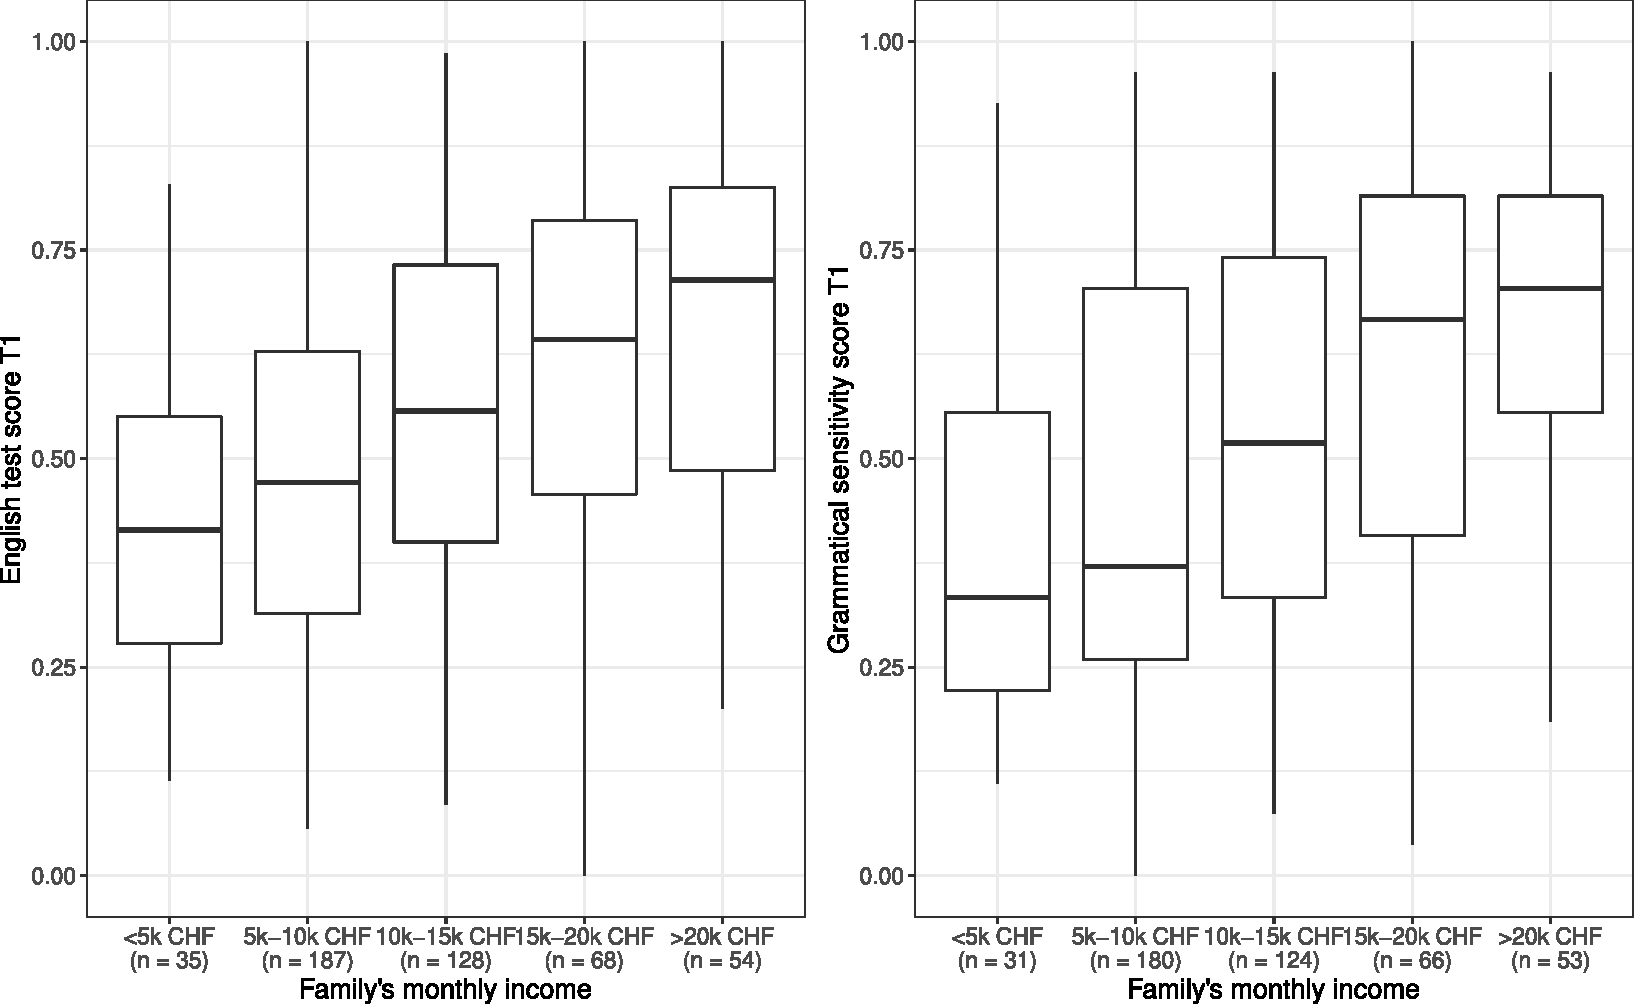
\includegraphics[width=\textwidth]{figures/Figure5.1.pdf}
\caption{Associations between earnings and a) English test score and b) Grammatical sensitivity score at T1. There are 66 missing answers for the income question in the left and 64 missing answers in the right panel.\label{fig:05:1}}
\end{figure}

The positive association of parental income and the development of language abilities comes as no surprise. The positive association between the socioeconomic status of a child’s family and their school performance has been widely investigated in the field of sociology of education (see \citealt{EntwisleAlexander1992} for a classic study on the topic, \citealt{FernaldEtAl2013} for a recent example on very early differentiation , \citealt{HäberlinEtAl2005} for an investigation of the Swiss situation).

Figures 5.1 a and b show monotonic associations between the parents’ income on the one hand and general proficiency in English at T1 and with language analysis as measured by the \textit{words in sentences} task of our adapted subtest from MLAT-E on the other hand. While the English score represents the main outcome variable of the researcher interested in foreign language learning, the MLAT-E subtest represents a classic, prototypical language aptitude measure. The Figures show that not only the skills themselves but also abilities underlying the development of such skills in the target language co-vary with income.

A second association -- and one that is often embraced in public debates on the multilingual curriculum -- concerns teaching foreign languages to children with an immigrant background who do not speak the local language in their families. Critics of the current multilingual curriculum that includes two compulsory foreign languages in primary school argue that in particular these second language learners are overwhelmed by the task of learning the local language and medium of instruction as well as two foreign languages such as English or French \citep{KüblerEtAl2014}. \figref{fig:05:2} shows the association of English scores with groups of children: (a) children who do or do not speak German as the only or one of their languages at home and (b) children who were born in Switzerland or abroad.

\begin{figure}
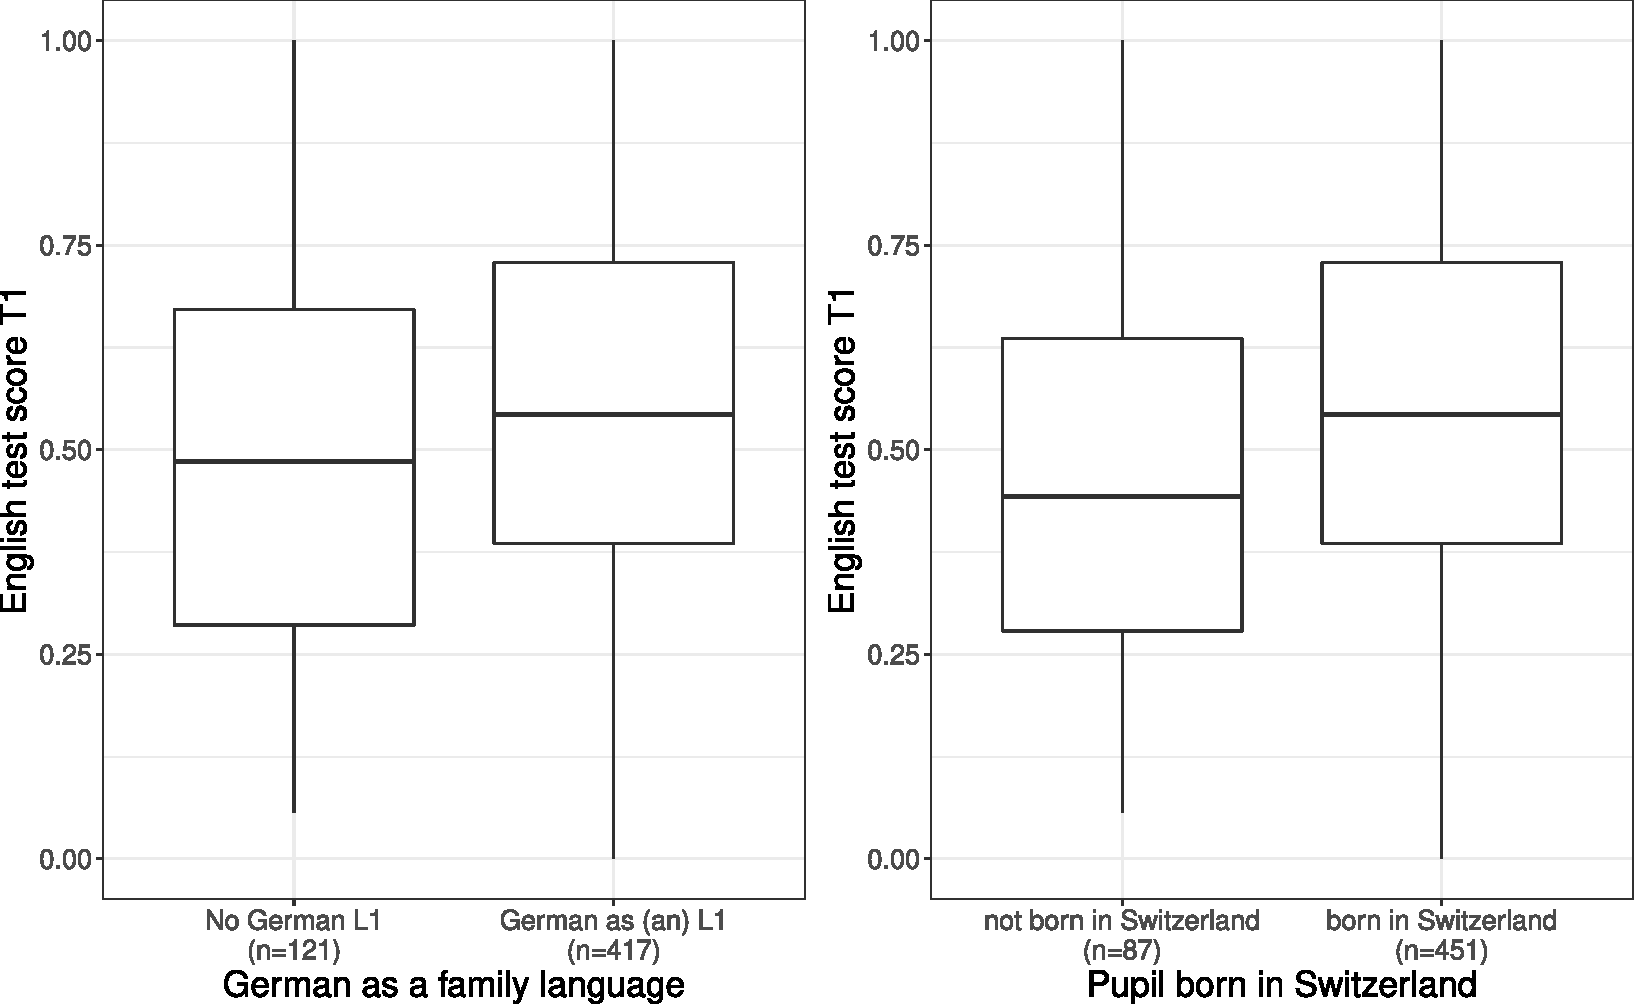
\includegraphics[width=\textwidth]{figures/Figure5.2.pdf}
\caption{English scores at T1 and either German as a home language (left) or country of birth of the children (right).\label{fig:05:2}}
\end{figure}

As expected, the central tendency for the German speakers and for the Swiss born children is higher, which seems to confirm the expectations expressed above.

In this chapter, I add information such as the four variables plotted in Figures 5.1 and 5.2, that is, information on the family background of the pupils in the LAPS-II data, to the analysis of language aptitude, cognitive and affective learner dispositions. In doing so, I use the operationalizations and the statistical modelling presented in Chapter 3. As in these previous analyses, children who speak English at home and who have spent substantial parts of their lives in an English-speaking context were excluded. In addition to the factors identified in Chapter 3, I add two constructs related to the individual background of each learner. These constructs are arguably systematically associated with language learning and cognitive abilities in general, as laid out in the next section. A more complicated structural equation model than the one discussed in Chapter 3 will therefore be fitted to the data of the first measurement point. The goal is to shed light on the associations between these additional background variables and the language-related constructs that are at the core of our inquiry.

\subsection{Social background and educational success}

This chapter focuses on explaining variance in English skills at the first measurement time in the LAPS-II project. In Chapter 4, we asked the question which factors allow us to predict skills in the target language at T3. When controlling for many potentially relevant factors, we found that English at T1 turns out to be the most informative predictor variable for these skills. Adding social information, however, does not increase the prognostic accuracy.

Sociolinguists and sociologists of education have accumulated a great wealth of evidence on the systematic associations of social class and language learning and use(see \citealt{AvineriJohnson2015} for an overview). Most of the evidence concerns first or second language learning, studies of the social conditioning of foreign language learning are relatively scarce (but see \citealt{Klieme2008} for a study that includes social information). If the influences on foreign language learning are similar to those observed in school learning in general, similar associations of the social background characteristics with the outcome variable are to be expected. 

The learning of two foreign languages in our primary school context is not an elite phenomenon. All children in state run schools and in private schools complying with the national curricula start learning two foreign languages during the primary school years. Our sample thus is not a self-selected sample of pupils following a special curriculum. 

As shown in the literature on inequalities in education, groups can be discriminated against based on their gender, social class, ethnicity or race (\citealt{LucasIrwin2018}). In our context, two particularly important categories are systematically confounded: Pupils from immigrant families speaking other languages than German at home tend to be pupils from low-income families, too \citep{Kronig2003}. As a consequence, pupils with a migrant background cumulate risk factors related to class and to language. Investigating additional language learning in these children means testing competing hypotheses from different fields: From the sociological point of view, immigrant children are expected to perform worse in school in general for the reasons spelled out above. From the point of view of third language acquisition theory, with the exception of pupils who start simultaneously learning both German as an L2 and English as L3,\footnote{Within the group of pupils who do not speak German as a family language, 3 out of 72 4\textsuperscript{th} graders and 2 out of the 49 5\textsuperscript{th} graders did not go to a German-language school in the Canton of Zürich the year before.} such learners are expected to have fewer problems learning an additional language since they have the necessary learning apparatus already up and running due to their previous second language learning experiences (\citealt{HerdinaJessner2002}).

Given these contradictory expectations from different disciplines, it is useful to test the impact of social status and L2 learner status in a comprehensive model.

\subsection{Educational, cultural and material indicators as background variables}

The background information used in this analysis consists of variables gathered via a parental questionnaire (see \tabref{tab:02:2} in Chapter 2 and Chapter 6 in \citealt{Vanhove2021} for more details). They encompass information on the origins and first languages of the parents as well as on economic and educational aspects of the families.

Socioeconomic status arguably should not simply be expressed via economic indicators such as the earnings used in \figref{fig:05:1}. An influential approach to status and its reproduction is the theory of different capitals proposed by \citet{Bourdieu1979}. Terms such as cultural and economic capital (among other types of capital) are used in different, evolving ways by Bourdieu himself and by other scholars, and it is impossible to give a detailed account of the theory of the different capitals here (see \citealt{Farkas2018} for a discussion citing the most recent literature). Bourdieu’s theorizing on the different instantiations of capital is rather complex and also controversially debated in sociology (see \citealt{Riley2017} for an example). I do not claim that mapping a handful of manifest variables to two constructs labelled \textit{economic} and \textit{cultural} \textit{capital} does justice to these debates. The insight, however, that social status and legitimacy is not only a matter of money certainly echoes parts of Bourdieu’s early thinking about dimensions, mechanisms, and resources mobilized in the reproduction of social inequalities. Analogous distinctions between material dispositions of study participants on the one hand and cultural and educational dispositions on the other are often made by scholars representing different disciplinary perspectives and thus, they seem  uncontroversial. On these grounds, it seems reasonable that the distinction should also inform the construction of the structural equation model in this chapter. In the remainder of this chapter, therefore, I will use the terms economic and cultural predispositions (\textit{econ\_p} and \textit{cult\_p}) to refer to two dimensions of the pupils’ family background.

\tabref{tab:05:1} lists the new variables used in the following analysis. The manifest variables operationalizing the constructs academic emotion (\textit{acad\_emo}) and \textit{cognition} are discussed in Chapter 3.

\begin{sidewaystable}
\caption{The background variables elicited with parents’ questionnaires that are used in this chapter\label{tab:05:1}}
\begin{tabularx}{\textwidth}{lQQ}
\lsptoprule
{Node label} & {Variable} & {Comment}\\\midrule
Swiss & Was the pupil born in Switzerland? & Switzerland the pupil’s country of birth (not citizenship)\\
educ\_f & Highest level of father’s education & Primary school, Secondary school, Apprenticeship, “Berufsmatura” (a higher vocational school leaving certificate),  Academic Maturity, Higher Vocational Education or University Degree\\
educ\_m & Highest level of mother’s education & \\
earnings & Family’s monthly income in CHF & (1) <5k, (2) 5--10k, (3)~10--15k, (4) 15--20k, (5)~>20k\\
bills & “Is there enough money to pay the monthly bills?” & 1 (not at all sufficient), 2 (rarely sufficient), 3 (sometimes sufficient), 4 (usually sufficient), 5 (always sufficient)\\
savings & “Is there enough money for saving?” & \\
holidays & “Is there enough money for travelling and holidays?” & \\
medical & “Is there enough money for medical and dental care?” & \\
books & “How many books are there in your household?” & (1) 0--10, (2) 11--25, (3) 26--100, (4) 101--200, (5) 201--500, (6) 500+\\
L1\_Ger & German (a) family language & Yes if German (a) family language\\
ParentsSwissBoth & Country in which pupil’s parents were born & Yes if both parents born in Switzerland\\
ParentSwiss &  & Yes if at least one parent born in Switzerland\\
\lspbottomrule
\end{tabularx}
\end{sidewaystable}

For further statistical treatment, all numeric variables were z-transformed, i.e., they were centered at their respective sample mean and then divided by their respective sample standard deviation. The participants were selected following these criteria (see Chapter 14 in \citealt{Vanhove2021} for details): no native speakers of English, no substantial exposure to English beyond school input, English T1 data available. This left a dataset of 538 pupils.

Based on these variables, it was possible to assess the impact of economic, cultural, and linguistic characteristics of the pupils’ families on the constructs at the core of the LAPS project and to answer the questions raised at the beginning of this chapter. 

\section{Modelling Strategy}

The data were modelled using the structural equation modelling function (sem()) of the lavaan package \citep{Rosseel2012} for R. Supplementary materials with the code and details of the analyses can be downloaded from \url{osf.io}.\footnote{\url{https://osf.io/kdxc7/?view_only=d6b0409de06f4d5cb82f2678471af56b}} The latent constructs are identical to the first and third factor in the confirmatory factor analysis described in Chapter 3 (cf. \figref{fig:05:1} in Chapter 3; see supplementary material to Chapter 3, modelling variant 4, for details). 

\begin{description}
\item[English:] English proficiency at T1 as measured by the OLYPT test. Two manifest scores are available, language use (‘use’) and listening comprehension (‘listening’).
\item[Academic emotion (\textit{acad\_emo}):] The same factor as the one described in Chapter 3; manifest measures of English self-concept (‘sel’), foreign language anxiety in the English classroom (‘anx’), and intrinsic motivation to learn English (‘int’).
\item[Cognition:] The same factor as the one described in Chapter 3; manifest measures of intelligence (‘iq’), visual and verbal working memory (‘vis’, ‘vem’), Phonetic coding ability (‘pho’), grammatical sensitivity (‘gra’), inductive ability (‘ind’), field independence (‘fie’), and German reading (‘ger’).
\end{description}

To this list I add two constructs related to the individual background of each learner (see variables listed in \tabref{tab:05:1}):

\begin{description}
\item[Economic predispositions (\textit{econ\_p}):] Manifest measures are ‘savings’, ‘bills’, ‘medical’, ‘holidays’, and ‘earnings’.
\item[Cultural predispositions (\textit{cult\_p}):] Manifest measures are ‘L1\_Ger’, ‘Swiss’, ‘books’, ‘educ\_f’, and ‘educ\_m’.
\end{description}

\subsection{Assumed causalities and correlations}

We expect the factor \textit{academic emotion} to be correlated with family background. Homes in which there is greater interest in culture, literature, and science arguably tend to foster more positive emotional conditioning towards school and learning in general, and most likely also towards learning English as a powerful vector of culture and science. We do not, however, assume a unidirectional causality from the background variables to the construct \textit{academic emotion} because there may be other constructs that we did not measure that influence both the background and the pupils’ emotional state regarding school and language learning. Moreover, based on the literature on educational sociology, it is reasonable to assume that there is a cyclic relationship between background and school performance, that is, pupils’ skills and learning processes are not simply a consequence of individual differences, but parents’ and teachers’ expectations as well as other mechanisms of educational systems have a measurable impact on them (see \citealt{JussimHarber2005} on expectancy or Pygmalion effects).

Although they emerged as two independent factors in the analysis of Chapter~3, the construct of \textit{academic emotion} is not completely orthogonal to the factor \textit{cognition}. Thus, it is reasonable to allow for a correlation between these two latent constructs. Cognition, in turn, is again supposed to be correlated with the family background, for the same reasons that apply to the family background and \textit{academic emotion}: As an example, we know from twin studies that achievement scores in foreign language, similarly to intelligence scores, can be explained in part by genetics (\citealt{RimfeldEtAl2015}, \citealt{Stromswold2001}). Thus, cognitive abilities and family background, while correlated, are not in a simple unidirectional causal relationship. 

English proficiency at T1 may be influenced by the aforementioned constructs. The impact of the two factors \textit{cognition} and \textit{academic emotion} has been established in the analysis in Chapter 3. The factor \textit{extrinsic motivation}, if \textit{cognition} and \textit{academic} \textit{emotion} are controlled for, is not a meaningful predictor of English skills and is thus not included in the present analysis. Family background as well as the family’s linguistic repertoire (e.g., German as a family language) may both directly and indirectly (via the two aforementioned factors) explain variance in English at T1. 

A first structural model is presented in \figref{fig:05:3}.\footnote{More information on all models, including path plots with standardized estimates, can be found in the online supplementary materials.} In this model, I assume only one construct capturing the socioeconomic and educational background of the parents (\textit{socioeco}). The variables capturing the first languages and the place where the child was born are added as manifest variables feeding into this construct. They arguably tap into relevant features of the family background: If the local language German is one of the family languages and if the child was born in Switzerland, then one can argue that the family is better lined up to conform with the educational system’s expectations.


\begin{figure}
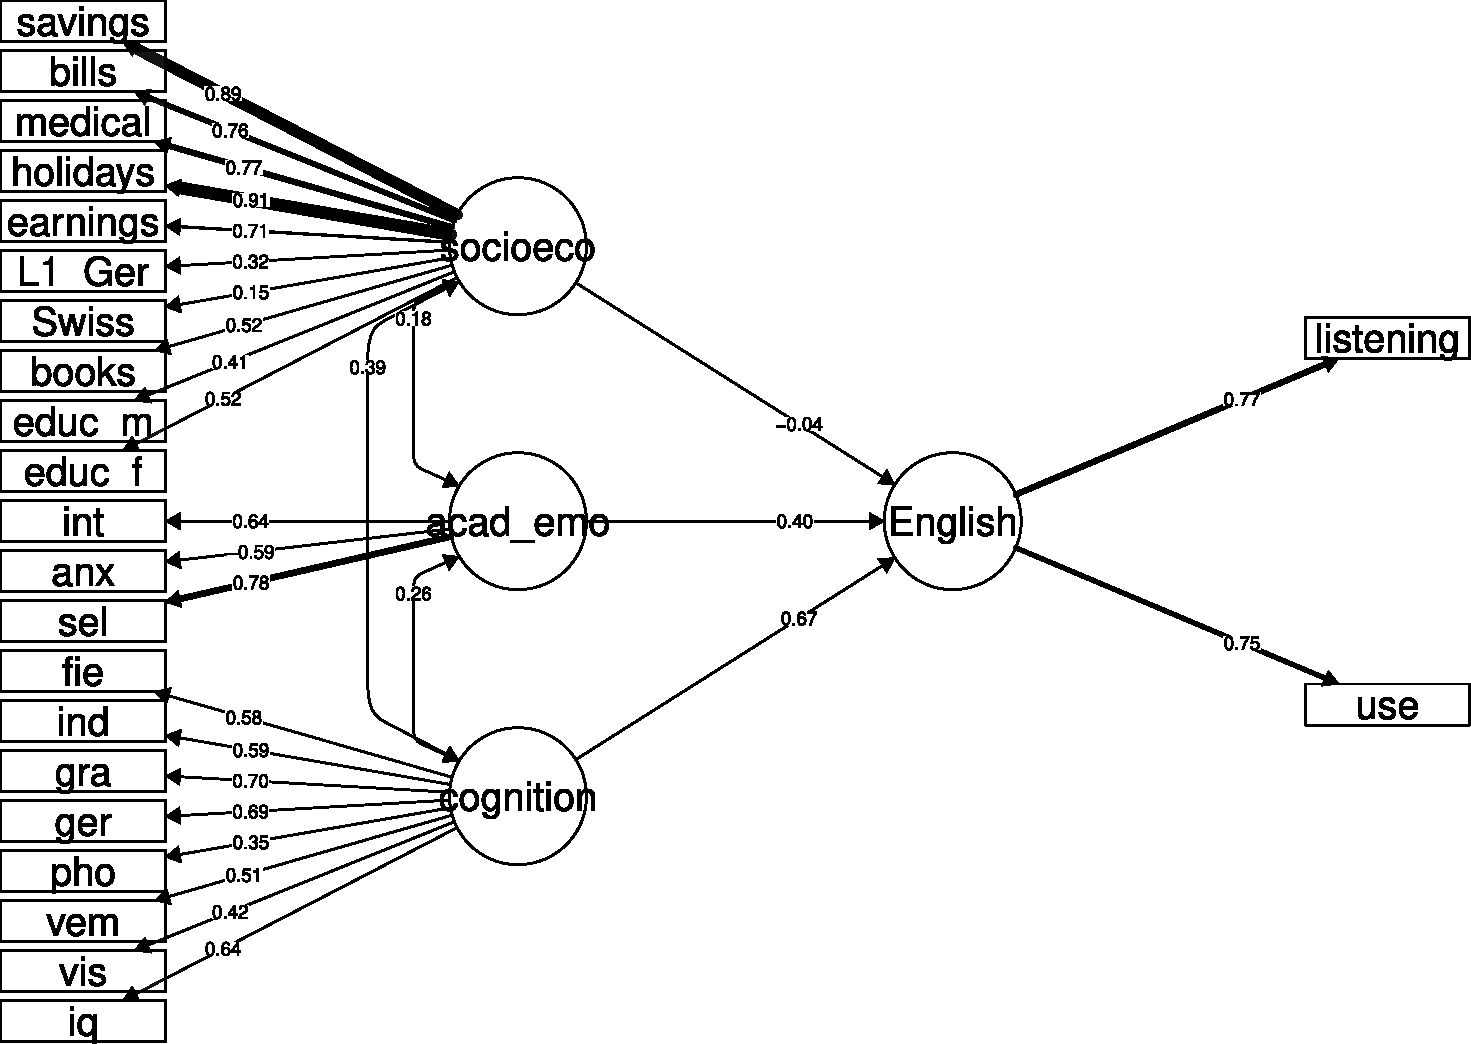
\includegraphics[width=\textwidth]{figures/Figure5.3.pdf}
\caption{The constructs and their assumed associations; variant A with only one construct for family background (viz., ‘socioeco’).\label{fig:05:3}}
\end{figure}

Based on the literature it is reasonable to have a somewhat more nuanced view on family background. As argued in the seminal work by \citet{Bourdieu1979}, social inequalities are more than a simple matter of economic resources. As I have argued earlier in this chapter, sociologists of education in the wake of Bourdieu thus use at least a two-dimensional space to locate groups with respect to economic and cultural predispositions, and scoring high on one of the two does not imply a high score on the other. The next, more realistic model thus includes two correlated constructs: \textit{cult\_p} to capture cultural predispositions (high values expressing higher affinity and proximity to the established ‘high’ culture) and \textit{econ\_p} to capture the economic resources. The first analysis in the next section will test whether assuming this more complicated model (\figref{fig:05:4}) is empirically justified.


\begin{figure}
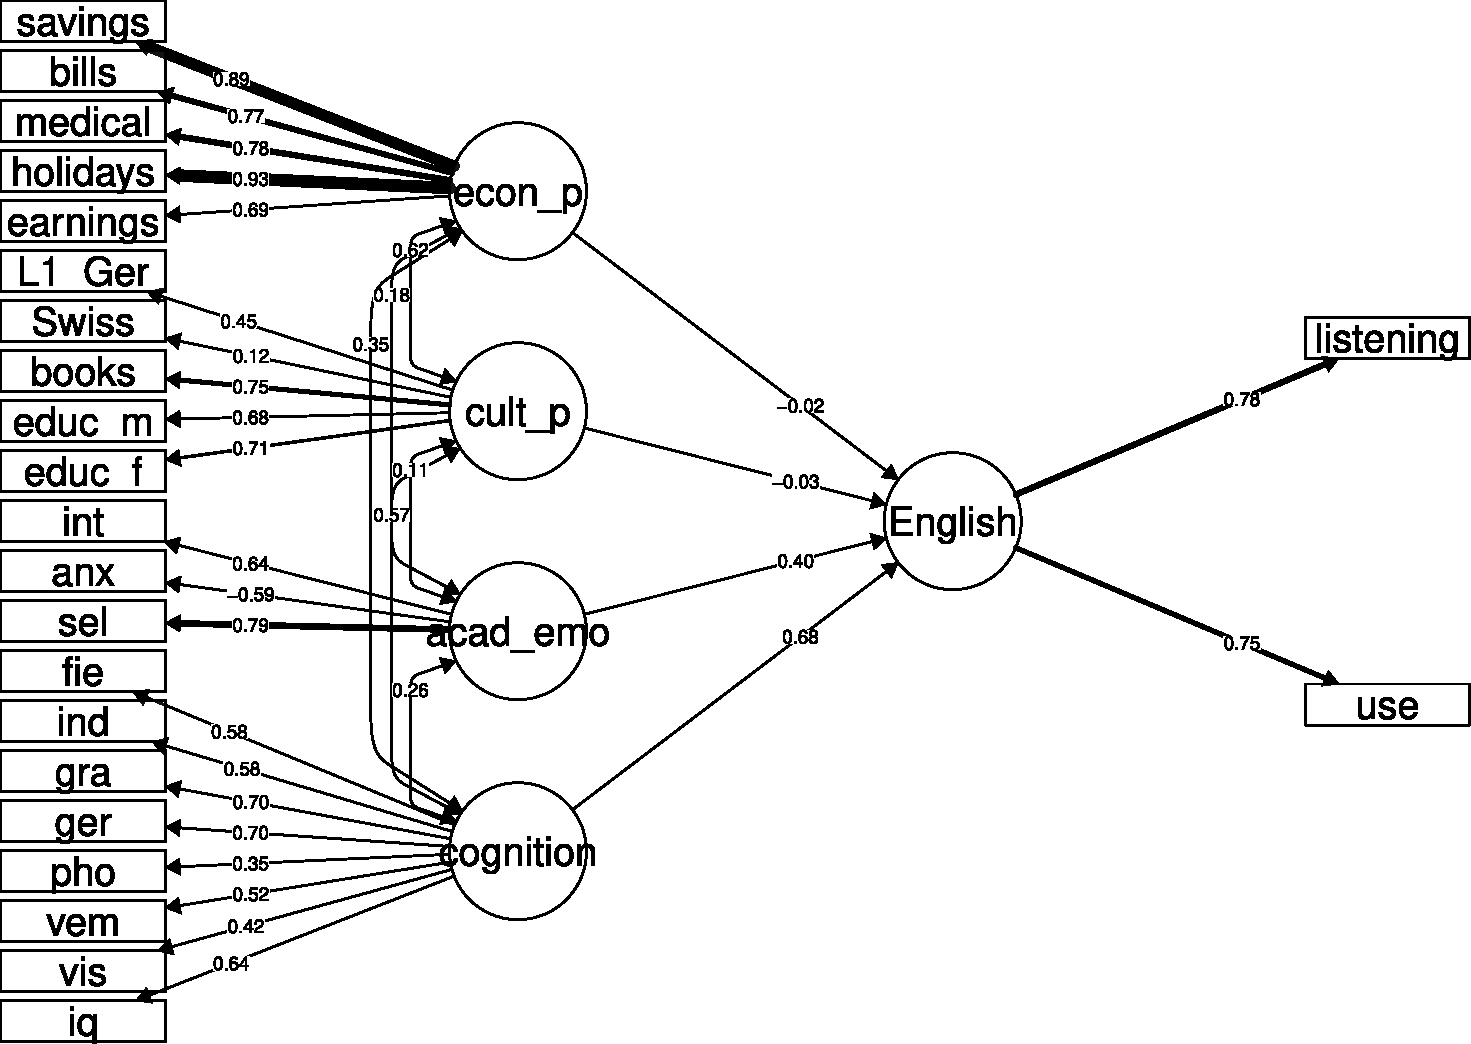
\includegraphics[width=\textwidth]{figures/Figure5.4.pdf}
\caption{The constructs and their assumed associations; variant B with two constructs for family background (viz., cult\_p and econ\_p). The figure includes the standardized estimates (see next section).\label{fig:05:4}}
\end{figure}

In the structural equation models fitted in this chapter I do not include any correlations between the residuals of the manifest variables.

In the next section different variants of the model are fitted to the data, and the optimal solution is selected based on fit indices and model comparisons.

\subsection{Socio-economic background: One or two dimensions}

The first analysis investigates whether one or two constructs are needed to capture the family background and its impact on the other constructs. The two models specified in Figures 5.3 and 5.4 are fitted to the data using the sem() function using the MLR estimator, which is suitable for clustered and incomplete data \citep{Rosseel2012}. The full output of these models can be obtained from the supplementary materials. \tabref{tab:05:2} compares these two models (and a few more models that will be discussed below) fitted in terms of three fit indices that are generally used to assess such models.

\begin{table}
\caption{Five different models fitted and three fit indices (root mean square error of approximation RMSEA, comparative fit index CFI, and standardized root mean residual SRMR).\label{tab:05:2}}
\begin{tabularx}{\textwidth}{lQ ccc}
\lsptoprule
\multicolumn{2}{l}{Model variant} & {RMSEA} & {CFI} & {SRMR}\\\midrule
A & one construct (socioeco) & 0.07 & 0.86 & 0.08\\
B & two constructs (econ\_p, cult\_p) & 0.05 & 0.93 & 0.06\\
C & two constructs and regression with German as a one of the native languages (L1\_Ger) & 0.05 & 0.93 & 0.06\\
D & two constructs and regression with the status of being born in Switzerland or not (Swiss) & 0.05 & 0.93 & 0.06\\
E & two constructs, no Swiss and L1\_Ger variables & 0.06 & 0.93 & 0.06\\
\lspbottomrule
\end{tabularx}
\end{table}



In a first step, I compare a model with one background construction to the model with two constructs social and economic predispositions (models A and B in \tabref{tab:05:2}; see supplementary materials, Table S5.2 for full details). The comparison of the models is a way to quantify the trade-off between model simplicity and its goodness of fit: Adding more predictors will almost unavoidably increase the model fit, but it also increases the danger of overfitting that model to the specific data set collected by the researcher. Comparing two information criteria (Akaike information criterion, AIC and Bayesian information criterion, BIC) of the alternative models helps us decide which one is preferable. The model with two constructs (B) has more parameters to be estimated and fewer degrees of freedom than the smaller model (A). The smaller model is nested within the larger model. The model with two constructs has better values for the relative model quality (the AIC and BIC indices are both lower, by 222 and 206 respectively), and the χ\textsuperscript{2}-test indicates that model with two latent constructs should be preferred (χ\textsuperscript{2} difference 202, $p<0.001$). We can therefore conclude that there is empirical support for the idea that different dimensions pertaining to the family background can be identified.

\subsection{Family origin and home languages}

After validating the two-dimensional nature of the family background, we address two other questions raised above: What is the influence of immigrant status and of other languages than German being spoken at home on the constructs under investigation? To assess these questions, the better model from the previous section is compared to two other models (see Figures 5.5 and 5.6).

The first comparison tests the prediction that not speaking German at home is an impediment to learning an additional language.  The assumption is that pupils who need to develop their L2 German at the same time as the foreign language English are overwhelmed by the learning task. The new model (C in \tabref{tab:05:2}) in \figref{fig:05:5} includes a regression arrow from the manifest variable L1\_Ger to English proficiency. This allows us to assess the degree of linear association of the two variables if all other variables are controlled for.

\begin{figure}
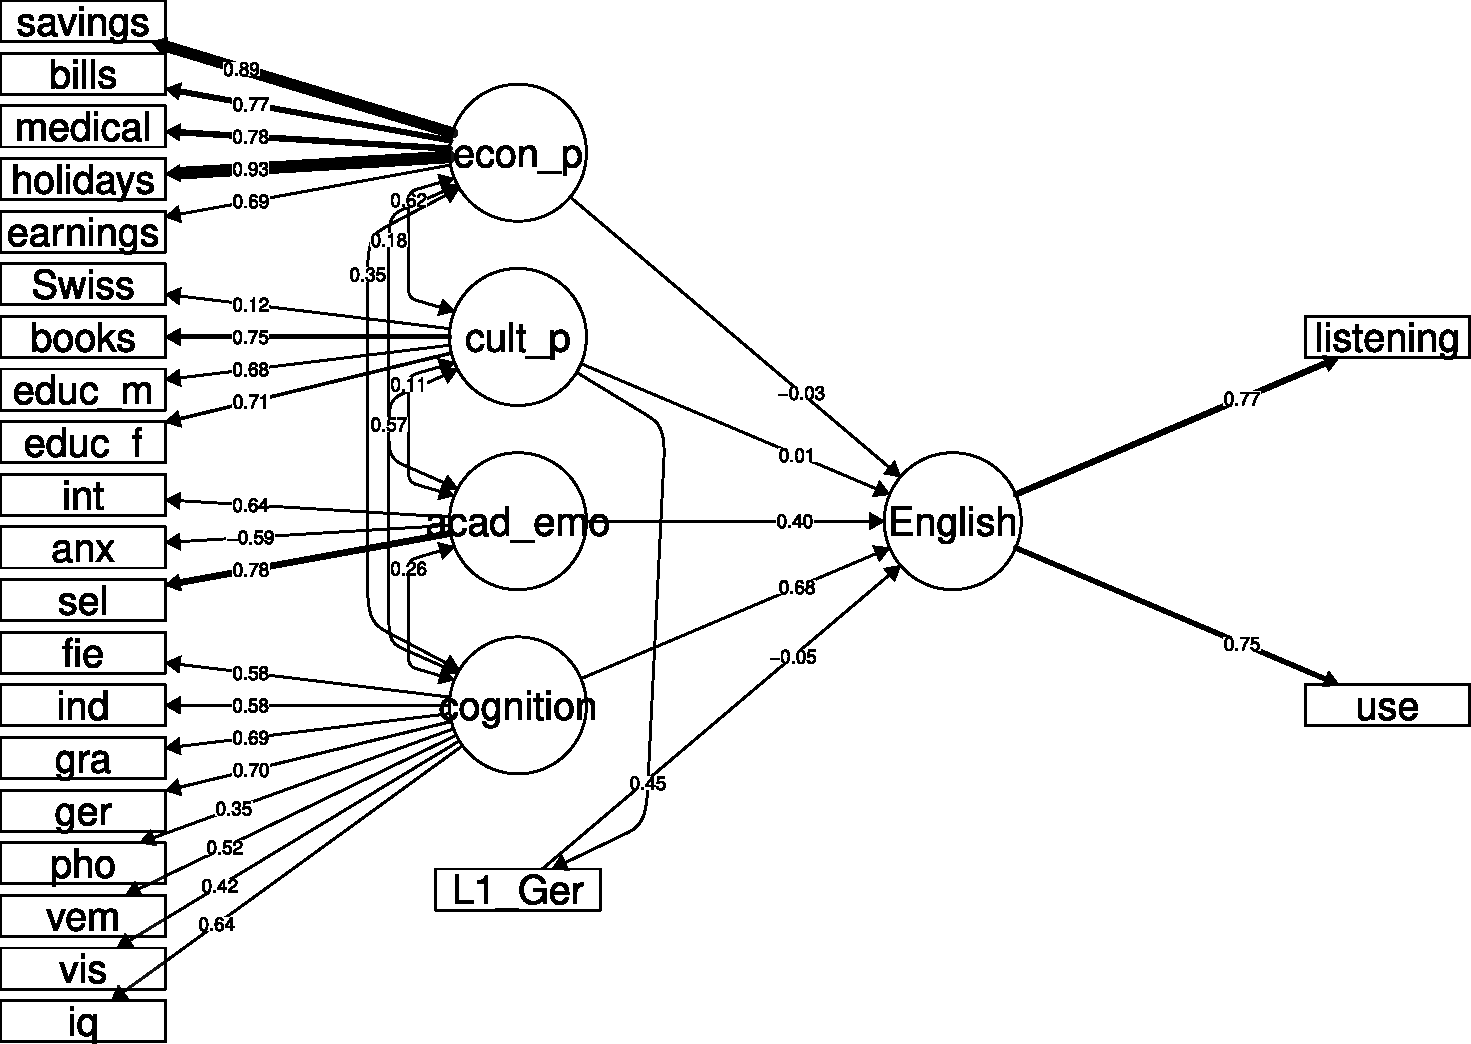
\includegraphics[width=\textwidth]{figures/Figure5.5.pdf}
\caption{Model C fitted to test the impact of being an L1 German speaker or not. The Variable L1\_Ger in this structural model affects English both directly and indirectly, first as a regressor and second via the latent construct of cultural predispositions.\label{fig:05:5}}
\end{figure}

The estimate for the regression from L1\_Ger to English is very small ($-0.052$), and the model comparison shows that adding this parameter to the structural equation model is not justified: The additional parameter leads to roughly similar AIC (+1) and BIC (+5) values, and the χ² difference is negligible (0.89, $p=0.35$; see Table S5.3 in the supplementary materials for full details).

We conclude that, when controlling for all other variables in the model, speaking German in the family or not does not account for much variability in English as a foreign language skills.

The second analysis follows an analogous logic. Policymakers worry about the difficulty for foreign-born pupils to learn both the local language and foreign languages in primary school, in particular if their home languages are typologically distant from the (European) languages used and taught at school. It is therefore useful to add the \textit{Swiss} variable (see \tabref{tab:05:1}) to test the impact of being born abroad or in Switzerland on English foreign language skills while controlling for all other variables.\footnote{Two other variants are possible and have also been tested: Both parents born abroad, one parent born abroad. All variants yield very similar results.} \figref{fig:05:6} shows the structural model (model D in \tabref{tab:05:2}) that includes an additional parameter estimate for this background variable.

\begin{figure}
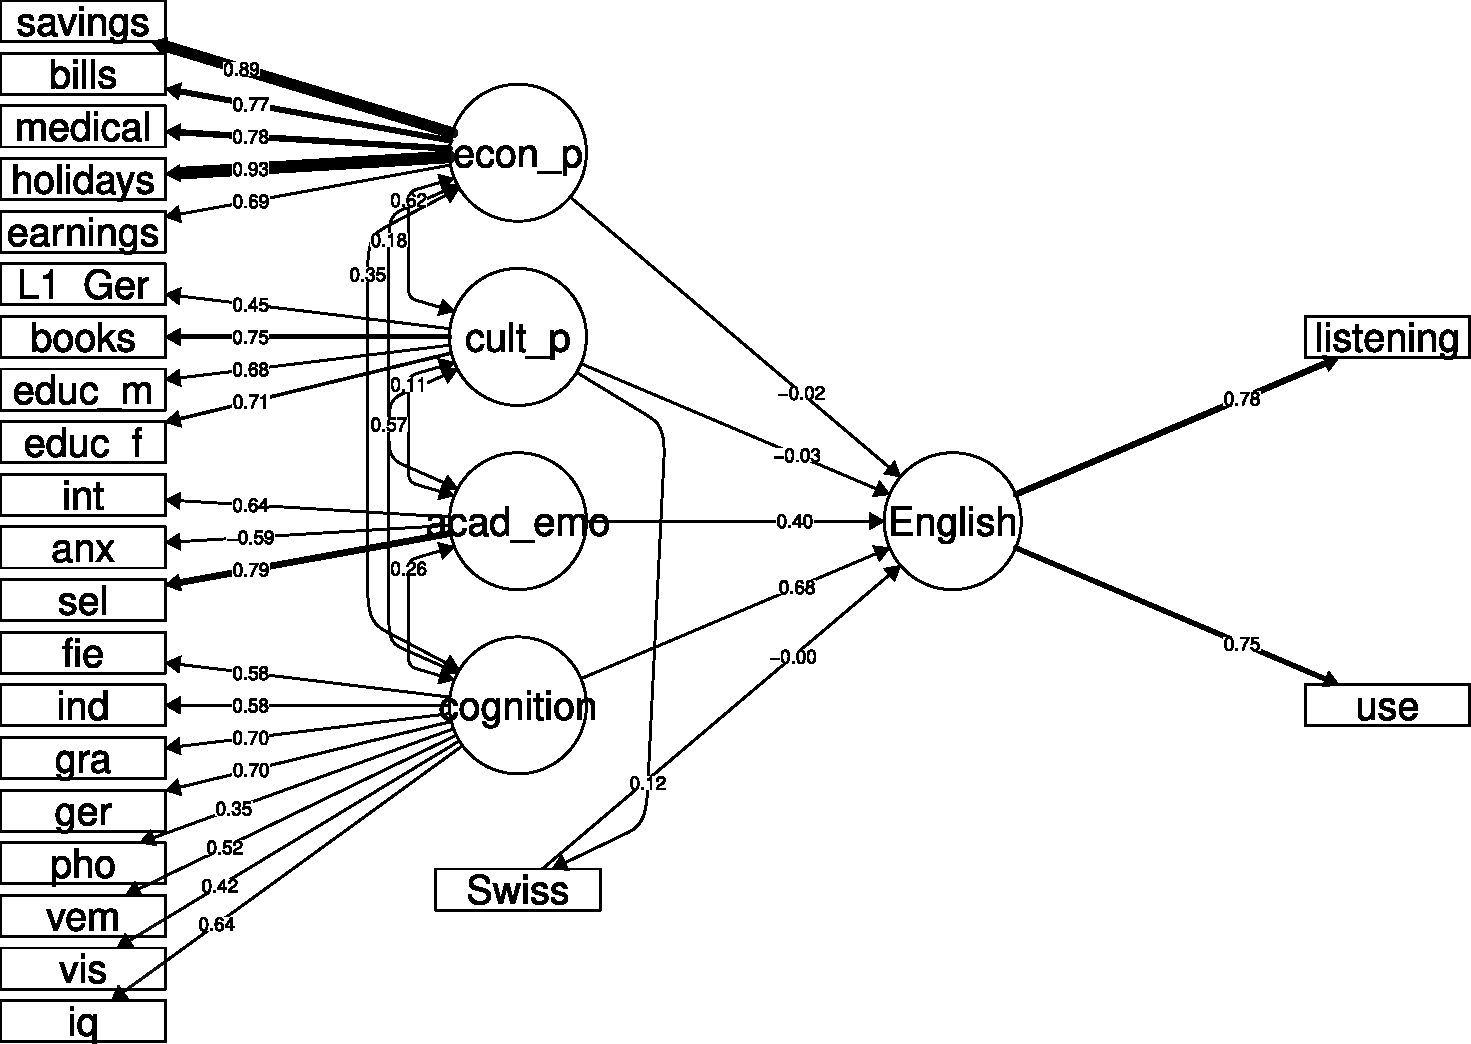
\includegraphics[width=\textwidth]{figures/Figure5.6.pdf}
\caption{Adding the variable Swiss (pupil born in Switzerland or not) to the structural equation (Model D). The variable \textup{Swiss} in this structural model affects English both directly and indirectly, first as a regressor and second via the latent construct of cultural predispositions.\label{fig:05:6}}
\end{figure}

Again, the standardized estimate for this additional regression is minute ($-0.002$). Adding this parameter to the structural equation model is not justified (AIC for the model with the additional estimate decreases by 2, BIC by 6, χ² difference is~0, see Table S5.4 in the supplementary materials for full details).

The two variables \textit{Swiss} and \textit{L1\_Ger} by themselves do not seem to be strongly associated with English skills. To assess how relevant they are to the overall model, I also fitted a simpler model similar to model A but that does not include these two variables. This last model (model E in \tabref{tab:05:2}) has only a slightly worse fit to the data.

\subsection{Discussion}

In the light of the comparisons above, we conclude that a model with two constructs for economic and cultural predispositions of the pupils’ families and the two factors \textit{cognition} and \textit{academic emotion} fits the data well. \figref{fig:05:5} shows its standardized estimates. These estimates do not change if one accounts for the clustered nature of the data using the lavaan.survey package as suggested by \citeauthor{Oberski2014} (\citeyear{Oberski2014}). For more detail refer to Figure S5.8 in the supplementary material.

The analysis shows, unsurprisingly in the light of the analyses in Chapter 3, that the two factors \textit{cognition} and, to a lesser extent, \textit{academic emotion}, are positively associated with English. Although the model allows the \textit{economic} and \textit{cultural} background constructs to directly influence English, the two corresponding estimates are very small (\textit{cult\_p}: $-0.03$, \textit{econ\_p}: $-0.02$). The impact of the two background constructs thus is predominantly indirect. English was not included in the \textit{cult\_p} construct since the overarching goal of our project is to investigate the favorable conditions and constraints on learning English as a foreign language. However, from a sociological point of view, language skills are undeniably part of the cultural resources of the families -- which is the reason why German language background was included in the construct (\figref{fig:05:5}). The analyses in this chapter are in line with this construal of language being part of the family’s cultural resources: the associations from cultural background and cognition, the latter being in turn an important predictor of English skills, can also be analyzed in this light.

\begin{table}
\caption{Correlations of four constructs in model B.\label{tab:05:3}}
\begin{tabular}{lcc}
\lsptoprule
factor & cult\_p & econ\_p\\\midrule
cognition & 0.57 & 0.35\\
acad\_emo & 0.12 & 0.18\\
\lspbottomrule
\end{tabular}
\end{table}



As shown in \figref{fig:05:4} and \tabref{tab:05:3}, the strongest associations emerge between cognition and cultural predispositions. To a somewhat lesser extent, economic predispositions are also positively associated with cognition. The two constructs operationalizing two dimensions of the family background thus are first and foremost associated with the cognitive abilities of the pupils. 

The literature on multilingual education often points out the incompatibility of the (often monolingual) habitus expected by Western educational systems with the attitudes of low-income and immigrant families. The term \textit{habitus} is borrowed from the Bourdieu approach, and typically authors in the field of intercultural studies and multilingual education advocate a new, different, multilingual \textit{habitus} that is hoped to make the educational systems a better place for minorities \citep{Gogolin1994}. Based on such assumptions, one would expect the association between these background variables and the attitudinal and emotional construct (\textit{acad\_emo}) to be important: Low-income migrant families would arguably foster attitudes that clash with the educational system’s expectations, and as a consequence children from such backgrounds should feel emotionally less at ease with respect to schooling and school subjects. In our data, it seems that this association is not particularly strong. This could either mean that expectations based on this habitus approach are not empirically borne out in the first place or that the schools under investigation have managed to overcome the differences implied by the habitus-based theory.

As a last sanity check preventing us from drawing hasty conclusions on the relative impact of being a migrant, we can fit the preferred model discussed here to different groups. As an example, the estimates can be compared across subgroups with one or two Swiss parents and the rest of the sample. Both variants yield very similar estimates across groups (see Figure S5.9. in the supplementary material). This supports the insight that once we account for the cognitive and affective individual differences as well as for the families’ socioeconomic and educational background, having a migrant background or not is not distinctive when it comes to the learning of English as a foreign language at school.

\section{Conclusion}

In this chapter, an additional source of individual differences was added to the variables already discussed in the previous chapters. Based on information about the pupils’ families’ educational and economic characteristics and their home languages, different structural equation models were fitted to the data.

The comparison of the fitted models shows that there is indeed a sound empirical basis for the classic distinction between economic and cultural predispositions of the participants. The analysis shows furthermore that these two constructs, if all other factors are held constant, are not directly associated with the foreign language skills. They are, however, associated with the two factors discussed in Chapter 3 -- most importantly with the construct that we termed \textit{cognition}. This construct involves not only memory and intelligence, but also language-specific components such as grammatical sensitivity, inductive learning, etc. I deliberately modelled a two-way relationship between cognition and academic emotion on the one hand and cultural predispositions on the other, since we know that other constructs that were not measured have an impact on both. The path leading from cultural and economic backgrounds to English skills via cognition, however, raises a few questions. Not only, so it seems, are smart children\footnote{I am aware that in the context of (language) pedagogy it is not fashionable to refer to smart and not-so-smart children. To some scholars in the field the mere idea of testing IQ, or sometimes testing any individual ability at all, seems problematic or scandalous (see \citealt[186]{Foucault1975} for an influential text in this respect). I certainly agree with the critique of abusive testing and the nefarious use of test scores in education (see \citealt{KuhnMai2015} for an example on language test scores in primary school), research, and politics. At the same time, I do not think that such abuse necessarily means that testing abilities is intrinsically bad. Ignoring robust evidence on individual differences in cognitive abilities simply because they are not compatible with one’s social and political ideologies is not only unscientific, but also problematic from the point of view of social policy. As \citet[chapter 9]{Plomin2019} argues, understanding individual differences, in particular if they are not caused by environmental biases, is not antithetical to the scholarly interest in equality and equal opportunity but on the contrary crucial for the assessment of such questions.} obviously more likely to achieve better in the foreign language, but these smart children are more likely to come from families with high cultural interests (that are often also economically well-off). One of the widely shared expectations is that educational systems should somehow manage to even out these inequalities and create more ‘equality of chances’, which boils down to comparable or almost equal skill levels at crucial moments of institutional selection (see \citealt{Heid1988} for a critical discussion of this postulate). If the schools in which the pupils in our sample are educated produced more equality in this sense, the association between the background variables and constructs such as cognition should be weak. But it is not. For T1, we diagnose an indirect association of family background on cognition and the emotional construct, which in turn has an impact on English skills. English skills at T1 furthermore are highly predictive of English skills at T3 (see Chapter 4). As far as our analyses allow any insight in the school’s potential to even out socially caused inequalities, they seem to be neither reduced nor exacerbated by the system. The latter would be the case if, on top of their advantage already visible at T1, social variables  explained additional variance beyond what is acquired and measured at T1 for the prediction of skills at T3. This, as Chapter 4 shows, is also not the case.

An impact of social background on school achievement would be completely unsurprising if the main object of investigation had been skills in mathematics or in the language of instruction, as was the case in \citet{Kronig2003}. However, according to the dominant view in multilingualism research (\citealt{Cenoz2003}, \citealt{HerdinaJessner2002}, \citealt{Montanari2019}), the subject we investigated is deemed to provide a headstart for a vulnerable subgroup of children: Immigrants who speak different languages at home should already have  gathered useful experience in learning new languages and should benefit from a multilingual boost (see \citealt{BertheleUdry2019} for references to studies with null or negative effects as well as an empirical investigation of this claim). It seems, at least in our data, that not even in a subject that should provide an advantage to pupils with an immigrant background such an effect can be found when controlling for the cultural and economic characteristics of the families.


\section*{Acknowledgments}
I would like to thank Alexandre Duchêne, Jan Vanhove and three anonymous reviewers for their invaluable comments on earlier versions of this chapter.

{\sloppy\printbibliography[heading=subbibliography,notkeyword=this]}
\end{document}
